\documentclass{article}

\usepackage[english]{babel}
\usepackage{csquotes}
\usepackage[letterpaper,top=2cm,bottom=2cm,left=3cm,right=3cm,marginparwidth=1.75cm]{geometry}

\newcommand{\currentversion}{1.11}

\usepackage{amsmath}
\usepackage{graphicx}
\usepackage{biblatex}
\usepackage{float}
\usepackage{multirow}
\usepackage[colorlinks=true, allcolors=blue]{hyperref}
\addbibresource{references.bib}
\title{
\includegraphics[width=0.8\textwidth]{MINI.png} \\ Project of Application for Piano Music Generation \\ by Artificial Intelligence Algorithms \\ [0.35em]\large Laboratory No. 1, \\ Version \currentversion }
\author{}
\date{}

\begin{document}
\maketitle
\begin{center}
    \normalsize\textbf{Authors:}
    \vskip10pt
    \Large{Szymon Górski} \\
    \large{Index No. 298796}
    \vskip10pt
    \Large{Weronika Piotrowska} \\
    \large{Index No. 305793}
    \vskip10pt
    \Large{Marcin Wojnarowski} \\
    \large{Index No. 303880}
    \vskip50pt
    \normalsize\textbf{Thesis Supervisor:}
    \vskip10pt
    \Large{Jerzy Balicki} \\
    \large{DSc, Associate Professor}
    \vfill
    \large{Warsaw, 2022}
\end{center}

\newpage
\begin{abstract}
    This document outlines the bachelor thesis project for the last semester of Computer Science and Information Systems at the Faculty of Mathematics and Information Science Warsaw University of Technology. Project assumptions and requirements are presented regarding the concept of generation music with Machine Learning techniques. Users can interact with the models through a user interface.
\end{abstract}

\vskip50pt
\section*{History of changes}
\begin{center}
    \begin{tabular}{ |p{0.07\textwidth} | p{0.1\textwidth} | p{0.5\textwidth} | p{0.21\textwidth}| }
        \hline
        Version         & Date       & Description                                                         & Author              \\
        \hline
        1               & 15.10.2022 & Initial creation of the document.                                   & Weronika Piotrowska \\
        \hline
        1.1             & 15.10.2022 & Added vocabulary, executive summary and non-functional requirements & Weronika Piotrowska \\
        \hline
        1.2             & 15.10.2022 & Added non-functional requirements.                                  & Weronika Piotrowska \\
        \hline
        1.3             & 16.10.2022 & Added user stories and functional requirements.                     & Marcin Wojnarowski  \\
        \hline
        1.4             & 16.10.2022 & Added document abstract.                                            & Marcin Wojnarowski  \\
        \hline
        1.5             & 16.10.2022 & Added SWOT analysis.                                                & Szymon Górski       \\
        \hline
        1.6             & 17.10.2022 & Added project schedule.                                             & Szymon Górski       \\
        \hline
        1.7             & 18.10.2022 & Added use-case descriptions.                                        & Marcin Wojnarowski  \\
        \hline
        1.8             & 18.10.2022 & Added motivation and goal description                               & Weronika Piotrowska \\
        \hline
        1.9             & 18.10.2022 & Added Gantt diagram.                                                & Szymon Górski       \\
        \hline
        1.10            & 18.10.2022 & Added work division.                                                & Szymon Górski       \\
        \hline
        \currentversion & 19.10.2022 & Added use case diagram.                                             & Marcin Wojnarowski  \\
        \hline
    \end{tabular}
\end{center}

\newpage


\tableofcontents
\newpage

\section{Introduction}
\subsection{Motivation}
Even though Artificial Intelligence is known for its various applications in majority of Information Sciences, the topic of music processing is not yet widely developed. Basing on existing solutions for image and video processing, we will implement and put in comparison three generative models. The motivation behind this project is to explore possible ways of music generation with the use of Machine Learning and to give this possibility to others by creating an user-friendly application that will show the effects of our work.

\subsection{Goals}

The aim of work is implementation and comparison of algorithms that can be used for music generation, as well as building an application, which will show the effects. We propose the following specification in order to achieve this goal. The specification includes descriptions of executive summary, functional requirements, along user stories and use cases, and non-functional requirements divided into URPS categories. To achieve our goal, we have designed a schedule of work presented in Gantt's diagram and division of work among project members. Finally, we present risk analysis prepared in a form of SWOT diagram.

\noindent
Optional goal is to generate a piece which is non-distinguishable from the original dataset. This issue, however, is mostly based on a subjective impression of an individual and is too complicated to be evaluated by a computer and will not be focused on in this project.

\section{Vocabulary}
\textbf{Artificial Intelligence} - The capacity of computers or other machines to exhibit or simulate intelligent behavior; the field of study concerned with this. Abbreviated AI. \cite{AI_OED}

\vskip5pt \noindent
\textbf{Machine Learning} - Machine learning is a branch of artificial intelligence (AI) and computer science which focuses on the use of data and algorithms to imitate the way that humans learn, gradually improving its accuracy. \cite{ML_IBM}

\vskip5pt \noindent
\textbf{Neural Network} - algorithmic structure, which is the core of deep learning algorithms; Their name and structure are inspired by the human brain, mimicking the way that biological neurons signal to one another. \cite{NN_IBM}

\vskip5pt \noindent
\textbf{LSTM} - Long Short-Term Memory; an artificial neural network used in the fields of artificial intelligence and deep learning. Unlike standard feedforward neural networks, LSTM has feedback connections. Such network can process not only single data points, but also entire sequences of data (such as recordings). \cite{LSTM}

\vskip5pt \noindent
\textbf{CNN} - Convolutional Neural Network; a neural network architecture using convolutional layers, which is advantageous in case of image processing. \cite{CNN}

\vskip5pt \noindent
\textbf{Markov Chain} - a stochastic model describing a sequence of possible events in which the probability of each event depends only on the state attained in the previous event. In this case, it will be referred to predicting next piano chords based on given number of previous chords. \cite{Markov}

\vskip5pt \noindent
\textbf{MIDI} - Musical Instrument Digital Interface. Standard file format describing notes being played at a given instant and how loud they are. As opposed to audio files, MIDI does not store actual audio.


\vskip5pt \noindent
\textbf{Acceptance criteria} - A set of conditions the system has to fulfill to be accepted by the user story agent (user/customer/admin). Once those are fulfilled, the user story can be considered as done and closed. Abbreviated AC.


\section{Specification}

\subsection{Executive summary}

The application will enable a user to upload their own audio files in MIDI format to train a selected model. Afterwards the user is able to generate a music sample generated by the model trained on the previously provided input. The program will base on Machine Learning algorithms, including LSTM and Convolutional Networks. The aim of the application is to provide an educational presentation of the performance of implemented models based on the given data.

\subsection{Functional requirements}

To begin, a strict set of requirements has to be defined. Most requirements are expressed as User Stories but we also provide a general list of requirements. A clear definition of requirements is crucial as it will be our main reference of our progress and will ensure that our system is complete and cohesive. The system will be split into three components, each with a separate responsibility: \textit{server}, \textit{client}, and \textit{model}.

\subsubsection{User stories}

\newcommand{\AC}{\subitem AC. }

\textbf{\large Model:}

Below are stories related to the \textit{model} component.

\begin{enumerate}
    \item
          As a user, I want to be able to process MIDI files.
          \AC Model component is able to read MIDI files and store them in a custom structure.

    \item
          As a user, I want to be able to train the a model with given input.
          \AC A function is exposed for each model which accepts input and trains the model.

    \item
          As an admin, I want to be able to track my model's performance.
          \AC Model saves training progress.
          \AC Training progress can be accessed and processed further.

    \item
          As an admin, I want to be able to test my model's performance.
          \AC Model can estimate its performance in a quantitative manner.

    \item
          As a user, I want to be able to save a trained model.
          \AC Model can be saved to a persistent medium.
          \AC Saved model is easily exportable to a different computer.

    \item
          As a user, I want to be able to load a saved model.
          \AC Model can be loaded from a persistent medium.
          \AC Model's performance is retained when loading the model.

    \item
          As a user, I want to be able to generate new music.
          \AC Model generates MIDI files based on a given seed.
\end{enumerate}


\textbf{\large Client \& Server:}

Below are stories related to the \textit{client} and \textit{server} component. User stories here describe the user perspective of interaction with the system however, these also entail some backend work as well.

\begin{enumerate}
    \item
          As a user, I want to be able to open a web page containing an app interface.
          \AC Web page displays some greeting interface.

    \item
          As a user, I want to be able to choose the target model.
          \AC UI presents a select field allowing to choose a model.
          \AC Once the choice has been made user can go to the next stage.

    \item
          As a user, I want to be able to pick either a pre-trained model or to train one myself.
          \AC User is presented with a choice between pre-trained and train yourself.
          \AC Once the choice has been made user can go to the next stage.

    \item
          As a user, I want to be able to upload MIDI files if I chose to train the model myself.
          \AC UI presents an option to choose a folder with MIDI files in it.
          \AC Files can be drag\&dropped for upload.
          \AC Files are sent to the backend server.

    \item
          As a user, I want to be able see the training progress.
          \AC A live-updating chart shows the training model performance.

    \item
          As a user, I want to be able to interrupt the training process so that I can start using the model immediately.
          \AC By pressing the interrupt button the training process stops.
          \AC User can move to the generation stage.

    \item
          As a user, I want to be able to generate music by providing a simple seed.
          \AC User can provide a music seed to start the generation process.
          \AC User can choose generated music length in seconds.
          \AC Generated music is saved to MIDI on the computer.
\end{enumerate}

\subsubsection{Use-case descriptions}

To be more specific, a list of core functional requirements as use cases is presented below.

\begin{center}
    \begin{tabular}{ |p{0.11\textwidth}|p{0.15\textwidth}|p{0.25\textwidth}|p{0.37\textwidth}| }
        \hline
        Actor     & Name                & Description                                 & System response                                                                                                                                                                                                   \\
        \hline
        \multicolumn{4}{|l|}{\textbf{Models}}                                                                                                                                                                                                                                                             \\
        \hline
        Developer & Model training      & Training a model with a given dataset       & Module creates a previously defined model and trains it with progress saving.                                                                                                                                     \\
        \hline
        Developer & Model evaluation    & Evaluating a model against given data       & Module creates loads a previously trained model and evaluates its performance after which the results are presented.                                                                                              \\
        \hline
        Developer & Music generation    & Generating music given a starting seed.     & Model accepts a seed and generates a sequence. This sequence is saved to a MIDI file.                                                                                                                             \\
        \hline
        Developer & MIDI parsing        & Being able to read and write MIDI files.    & System can read MIDI files and process to our needs. System can create MIDI files from model outputs.                                                                                                             \\
        \hline
        \multicolumn{4}{|l|}{\textbf{Server}}                                                                                                                                                                                                                                                             \\
        \hline
        Developer & Model integration   & Server and model components are integrated. & Server component can query models for various things (training, evaluation, generation) and receives back responses.                                                                                              \\
        \hline
        Developer & API                 & Server exposes an API.                      & Client receives responses from the server regarding queries and commands.                                                                                                                                         \\
        \hline
        Developer & File streaming      & Streaming files from and to a client.       & Client can download a file from the server. Server receives streamed files from the client.                                                                                                                       \\
        \hline
        \multicolumn{4}{|l|}{\textbf{Client}}                                                                                                                                                                                                                                                             \\
        \hline
        User      & Model configuration & Configuration of target model               & Buttons and switches are shown on the UI to allow for choosing the model and training status (pre-trained/new).                                                                                                   \\
        \hline
        User      & File upload         & Uploading local files to the server         & Application accepts MIDI files to be uploaded. Files are sent to the backend server as the input dataset.                                                                                                         \\
        \hline
        User      & Model training      & Training a selected model                   & Server communicates with the models in order to train them. Server streams training progress back to the client. Client displays training progress in the form of live-updating charts and/or standalone scalars. \\
        \hline
        User      & Music generation    & Using a model to generate music             & Server communicates with the models in order to generate music sequences. Server sends a MIDI file back to the client. Client downloads the generated MIDI file.                                                  \\
        \hline
    \end{tabular}
\end{center}

\newpage
\subsubsection{Use case diagram}

Since most of the functionality will be on the side of designing and creating models which is behind the scenes, the use case diagram can be neatly summarized to the main features.


\begin{figure}[H]
    \centering
    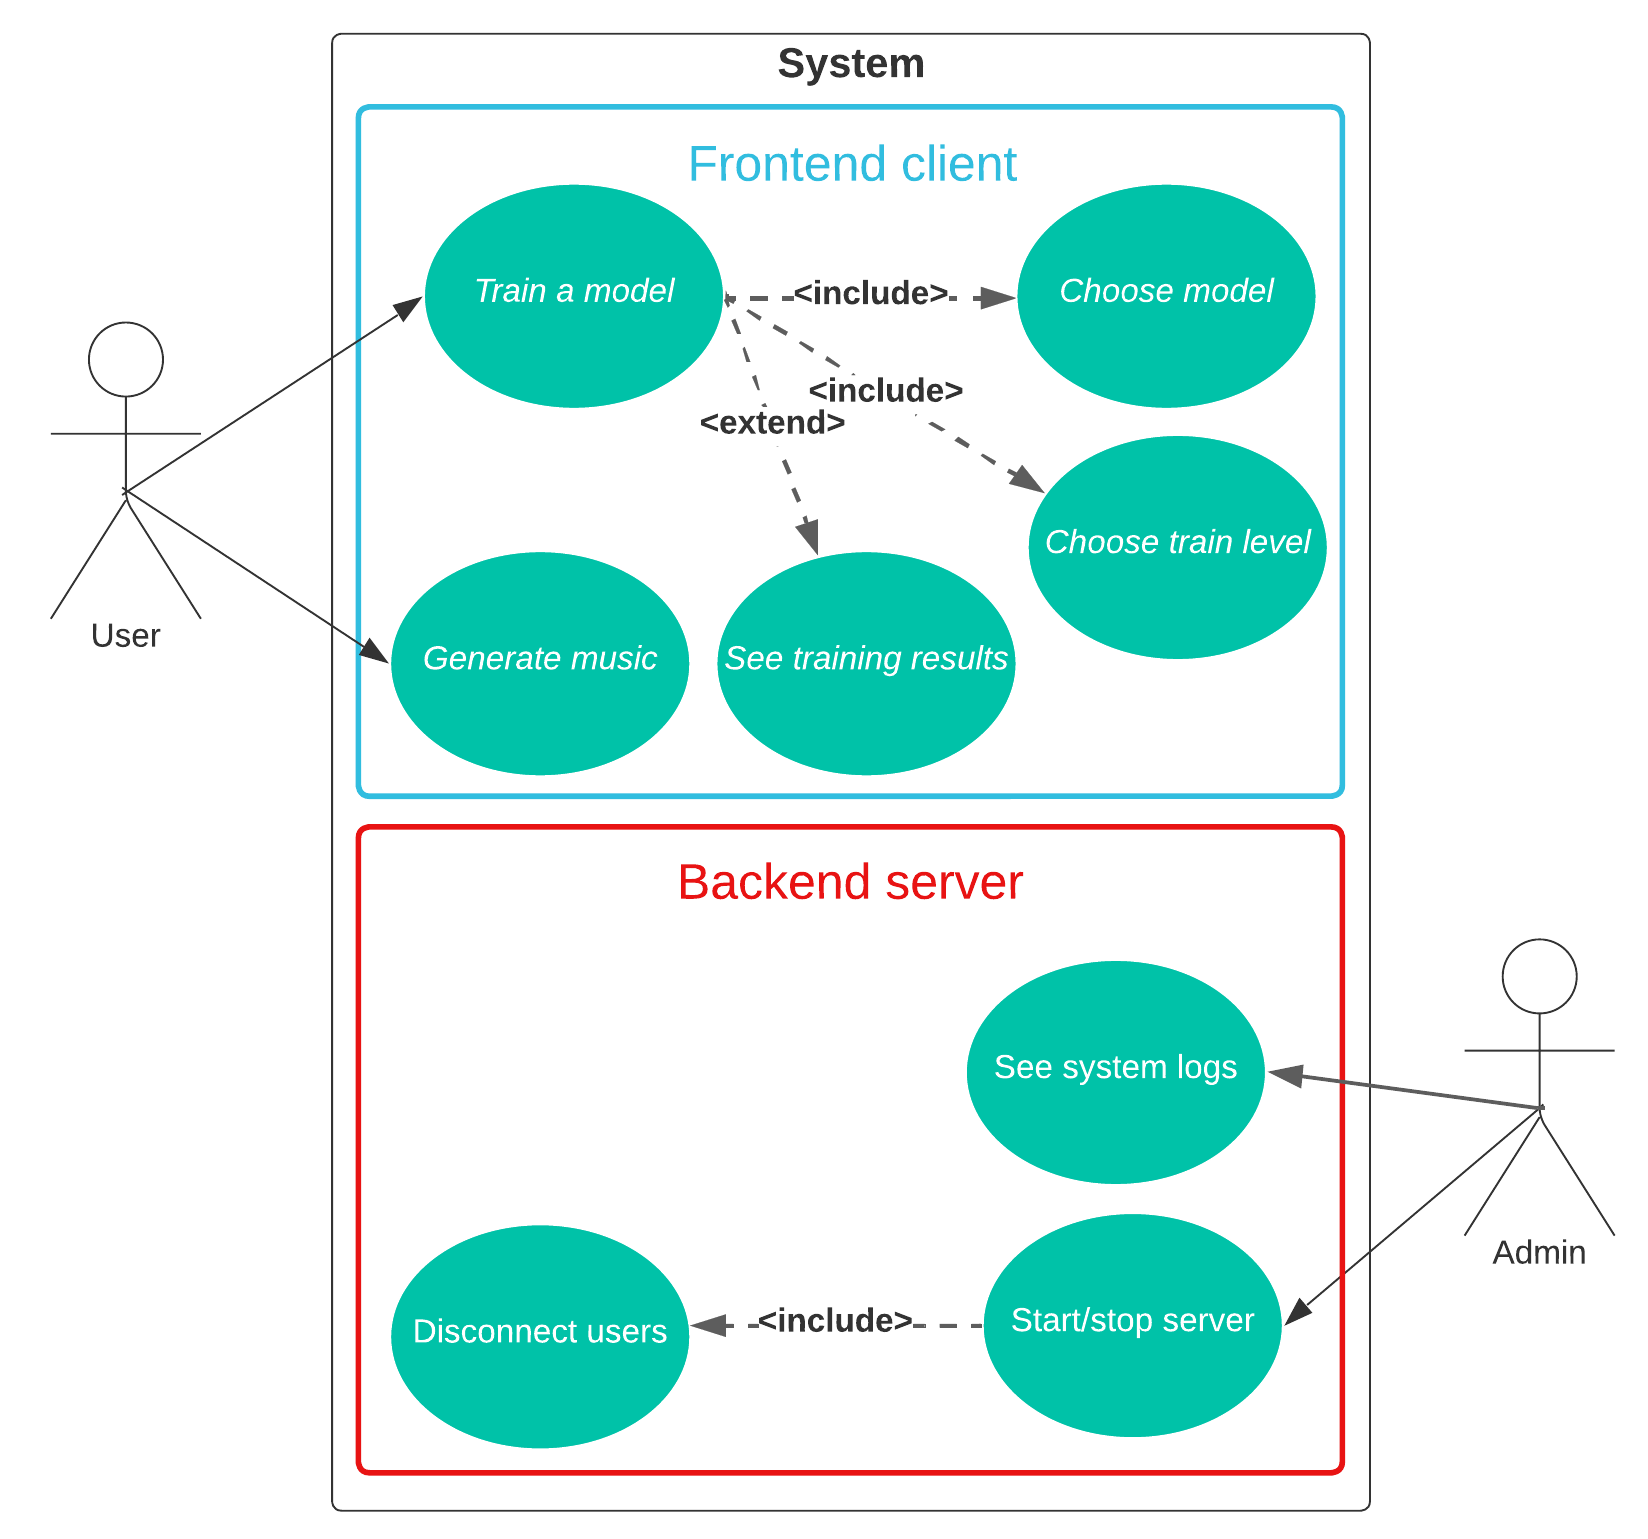
\includegraphics[width=0.7\textwidth]{use_case_diagram.png}
    \caption{Use case diagram for the user and admin interacting with the system.}
    \label{fig:use-case-diagram}
\end{figure}

\subsection{Non-functional requirements}
Below are examples of non-functional requirements grouped into individual URPS (Usability, Reliability, Performance, Supportability) categories:

\begin{center}
    \begin{tabular}{ |p{0.15\linewidth}|p{0.13\linewidth}|p{0.6\linewidth}| }
        \hline
        Requirements area                 & Requirement No. & Description                                                                                                                                                              \\
        \hline
        \multirow{3}{1em}{Usability}      & 1               &
        The application window must fit into a single screen of standard size (minimum 1920 x 1080 px)                                                                                                                                 \\
        \cline{2-3}
                                          & 2               & The application must be clear and legible, with font size not smaller than 10. All images and graphs displayed in the application must not be compressed in the runtime. \\
        \cline{2-3}
                                          & 3               & File upload must be working regardless of operating system.                                                                                                              \\
        \hline
        \multirow{1}{4em}{Reliability}    & 4               & The application must be available at least 99\% of the time, with exception of server service breaks.                                                                    \\
        \hline
        \multirow{2}{4em}{Performance}    & 5               & The application should provide exchange of information between user and server in no longer than 3 seconds.                                                              \\
        \cline{2-3}
                                          & 6               & When training a model, the application should update on its progress.                                                                                                    \\
        \hline
        \multirow{2}{4em}{Supportability} & 7               & The application must be backwards compatible with all of its components.                                                                                                 \\
        \cline{2-3}
                                          & 8               & In case of any exception, the application should provide a detailed information to the user.                                                                             \\
        \hline
    \end{tabular}
\end{center}

\section{Project schedule}
\subsection{Scope of work}
The following table presents division of the project into parts and tasks with their respective time necessary to finish each assignment. Six main parts of the project were separated due to their subject.

\begin{center}
    \begin{tabular}{ |p{0.13\linewidth}|p{0.55\linewidth}|p{0.20\linewidth}| }
        \hline
        Part No.                                                                & Task                                                 & Duration (weeks) \\
        \hline
        \multicolumn{2}{|l|}{\textbf{1. Project preparation}}                   & \textbf{10}                                                             \\
        \hline
        1.1                                                                     & Research and study on the thesis' topic              & 4.5              \\
        \hline
        1.2                                                                     & Research and study on available algorithms and tools & 4.5              \\
        \hline
        1.3                                                                     & Choice of the AI algorithms and the technology stack & 1                \\
        \hline
        \multicolumn{2}{|l|}{\textbf{2. Data management}}                       & \textbf{6}                                                              \\
        \hline
        2.1                                                                     & Research of available datasets                       & 3                \\
        \hline
        2.2                                                                     & Choice of datasets to be included and accessing them & 1                \\
        \hline
        2.3                                                                     & Implementation of MIDI transcription module          & 2                \\
        \hline
        \multicolumn{2}{|l|}{\textbf{3. 1st model development}}                 & \textbf{5}                                                              \\
        \hline
        3.1                                                                     & Model implementation                                 & 3                \\
        \hline
        3.2                                                                     & Model evaluation                                     & 1                \\
        \hline
        3.3                                                                     & Model testing and tuning                             & 1                \\
        \hline
        \multicolumn{2}{|l|}{\textbf{4. 2nd model development}}                 & \textbf{5}                                                              \\
        \hline
        4.1                                                                     & Model implementation                                 & 3                \\
        \hline
        4.2                                                                     & Model evaluation                                     & 1                \\
        \hline
        4.3                                                                     & Model testing and tuning                             & 1                \\
        \hline
        \multicolumn{2}{|l|}{\textbf{5. Client-server application development}} & \textbf{4}                                                              \\
        \hline
        5.1                                                                     & Client-server application establishment              & 2                \\
        \hline
        5.2                                                                     & Graphic User Interface design and implementation     & 1                \\
        \hline
        5.3                                                                     & Application integration with both AI models          & 1                \\
        \hline
        \multicolumn{2}{|l|}{\textbf{6. Testing}}                               & \textbf{4}                                                              \\
        \hline
        6.1                                                                     & Unit testing                                         & 1                \\
        \hline
        6.2                                                                     & Integration testing                                  & 1                \\
        \hline
        6.3                                                                     & System testing                                       & 1                \\
        \hline
        6.4                                                                     & Efficiency and quality comparison of both AI models  & 1                \\
        \hline
        6.5                                                                     & Final corrections and system review                  & 1                \\
        \hline
    \end{tabular}
\end{center}

\subsection{Gantt diagram}
The following pictures represent a Gantt diagram locating assignments in a timetable. It also represents dependencies between particular tasks presented above.

\begin{center}
    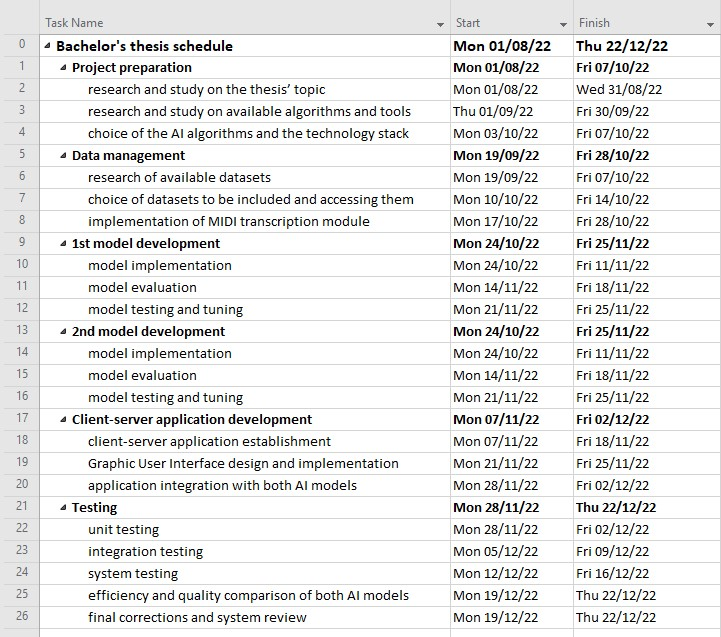
\includegraphics[width=0.7\textwidth]{Gantt_1.jpg} \\
    \textit{Part 1:} List of tasks with their respective dates of staring and finishing
    \vskip10pt \noindent
    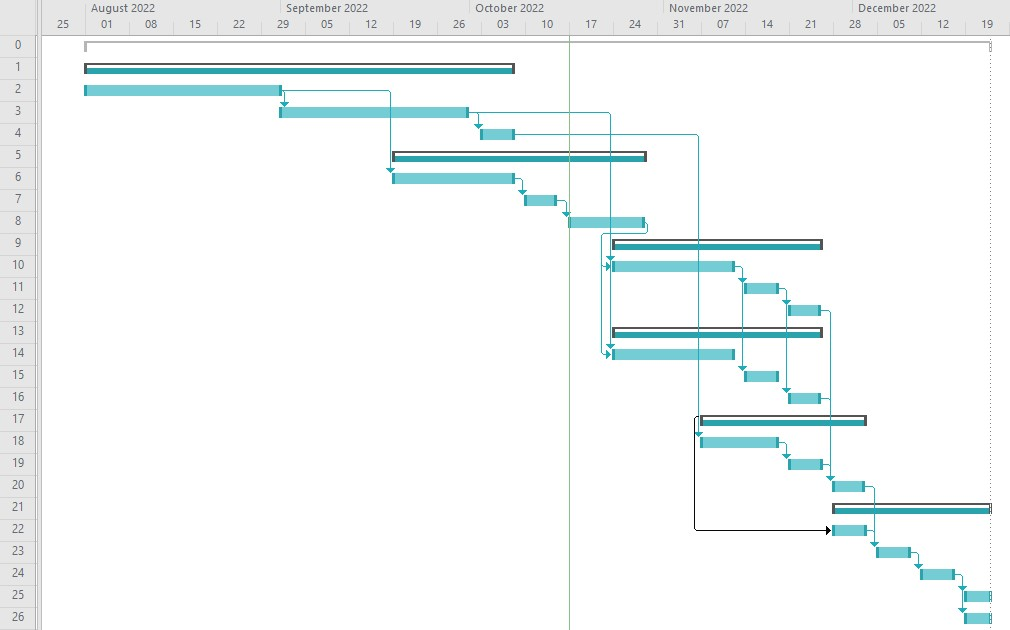
\includegraphics[width=1\textwidth]{Gantt_2.jpg} \\
    \textit{Part 2:} Diagram of tasks and their dependencies against time \\ (as of 17 October 2022, represented by a green line)
\end{center}

\subsection{Work division}
The following table shows the distribution of tasks among the authors. The division was designed to provide equal allocation of work as well as its continuity of performance. Some work should be or already have been done by all together - these assignments were presented under 'collective tasks'.

\begin{center}
    \begin{tabular}{ |p{0.23\linewidth}|p{0.67\linewidth}| }
        \hline
        Author                                           & Tasks         \\
        \hline
        \multirow{3.75}{10em}{\textit{Collective tasks}} &
        \begin{itemize}
            \item [1.] Project preparation
            \item [2.1.] Research of available datasets
            \item [6.5.] Final corrections and system review
        \end{itemize}                  \\
        \hline
        \multirow{3.75}{10em}{Szymon Górski}             &
        \begin{itemize}
            \item [2.2.] Choice of datasets to be included and accessing them
            \item [2.3.] Implementation of MIDI transcription module
            \item [4.] 2nd model development
            \item [5.2.] Graphic User Interface design and implementation
            \item [6.1.] Unit testing
        \end{itemize} \\
        \hline
        \multirow{3.75}{10em}{Weronika Piotrkowska}      &
        \begin{itemize}
            \item [3.] 1st model development
            \item [5.2.] Graphic User Interface design and implementation
            \item [5.3.] Application integration with both AI models
            \item [6.3.] System testing
            \item [6.4.] Efficiency and quality comparison of both AI models
        \end{itemize}  \\
        \hline
        \multirow{3.75}{10em}{Marcin Wojnarowski}        &
        \begin{itemize}
            \item [4.] 2nd model development
            \item [5.1.] Client-server application establishment
            \item [5.3.] Application integration with both AI models
            \item [6.2.] Integration testing
        \end{itemize}          \\
        \hline
    \end{tabular}
\end{center}

\newpage
\section{Risk analysis}
A risk analysis of the project was done using the 'SWOT' methodology. The result is presented in the following table.

\begin{center}
    \begin{tabular}{ |p{0.15\linewidth}|p{0.365\linewidth}|p{0.365\linewidth}| }
        \hline
        \multicolumn{1}{|c|}{\textbf{SWOT}}                                                                                                              & \multicolumn{1}{|c|}{HELPFUL}                 & \multicolumn{1}{|c|}{HARMFUL}              \\
        \hline
                                                                                                                                                         &                                               &                                            \\
        \multicolumn{1}{|c|}{INTERNAL}                                                                                                                   & \multicolumn{1}{|c|}{\textbf{Strengths:}}     & \multicolumn{1}{|c|}{\textbf{Weaknesses:}} \\
                                                                                                                                                         &
        \begin{enumerate}
            \item One of the authors has experience in developing music-generating AI systems,
            \item Possibility of consultation of solution design with people experienced in the field of music generation and AI (e.g., Project Supervisor),
            \item Extensive coverage of capabilities of used tools both in documentations and on the Internet,
            \item Multiple sets with MIDI files available in free domain,
            \item Good communication skills and motivation of all authors.
        \end{enumerate} &
        \begin{enumerate}
            \item Short period of time dedicated to developing core functions, while some learning algorithms may require significant amount of time to perform its tasks,
            \item Quality of results cannot be predicted straightforwardly,
            \item Impossibility of generating a MIDI set by one's own - the project depends on works by external authors,
            \item Large size, quality, and feature differences among different MIDI sets.
        \end{enumerate}                                                                                 \\
        \hline
                                                                                                                                                         &                                               &                                            \\
        \multicolumn{1}{|c|}{EXTERNAL}                                                                                                                   & \multicolumn{1}{|c|}{\textbf{Opportunities:}} & \multicolumn{1}{|c|}{\textbf{Threats:}}    \\
                                                                                                                                                         &
        \begin{enumerate}
            \item Raise of competence in the field of Artificial Intelligence,
            \item Possibility of further development of the project (e.g., as a master's thesis),
            \item Possibility of publishing the project on the Internet and gaining users (similarly to other AI projects e.g., DALL-E and its derivatives).
        \end{enumerate} &
        \begin{enumerate}
            \item Simultaneous completion of multiple projects throughout the semester,
            \item Some functionalities regarding learning algorithms may prone to fail or take too long to complete due to unsatisfactory (substandard) parameters of a user's PC,
            \item Consecutive development of the solution may happen in different periods than defined in the university's curriculum due to the need to focus on AI algorithms.
        \end{enumerate}                                                                         \\
        \hline
    \end{tabular}
\end{center}

\newpage
\printbibliography

\end{document}
